\documentclass[12pt]{article}
\usepackage[utf8]{inputenc}
\usepackage[english]{babel}
\usepackage[a4paper]{geometry}
%\geometry{top=1.5cm, bottom=1.0cm, left=1.25cm, right=1.25cm}
\usepackage{pdflscape}
\usepackage{xcolor}
\usepackage{tikz}
\usetikzlibrary{positioning, shapes.multipart}

\begin{document}
\title{Ejercicios de PERT}
\author{Ana Maritza Bello Yañez}
\maketitle
%\setlength{\parindent}{0pt}
%\setlength{\parskip}{1em}


\section{Ejercicio 1}
La empresa SALMA está preparando la planificación, aplicando la técnica PERT, de
un proyecto informático, cuyas actividades se indican en la tabla inferior, así
como sus precedentes y la duración expresada en semanas (optimista, pesimista y
más probable):  \\
\\

\begin{center}
\begin{tabular}{ccp{0.125\linewidth}p{0.125\linewidth}p{0.125\linewidth}}
Actividad &   Precedentes   &   Estimación optimista    &   Estimación probable
&   Estimación pesimista \\
\hline
A   &    -   &   1   &   2   &   3   \\
B   &    A   &   2   &   4   &   6   \\
C   &   B,H  &   1   &   1   &   1   \\
D   &    -   &   3   &   6   &   9   \\
E   &    G   &   2   &   3   &   4   \\
F   &    E   &   3   &   5   &   7   \\
G   &    D   &   1   &   2   &   3   \\
H   &    G   &   1   &   2   &   3   \\
I   &    D   &   1   &   3   &   5   \\
J   &    I   &   3   &   4   &   5   \\
K   &    D   &   2   &   3   &   4   \\
L   &   J,K  &   3   &   5   &   7   \\
M   &   C,L  &   1   &   2   &   3   \\
\end{tabular}
\end{center}

\begin{itemize}
    \item Diseño completo del grafo, incluyendo holguras y camino crítico.
    
    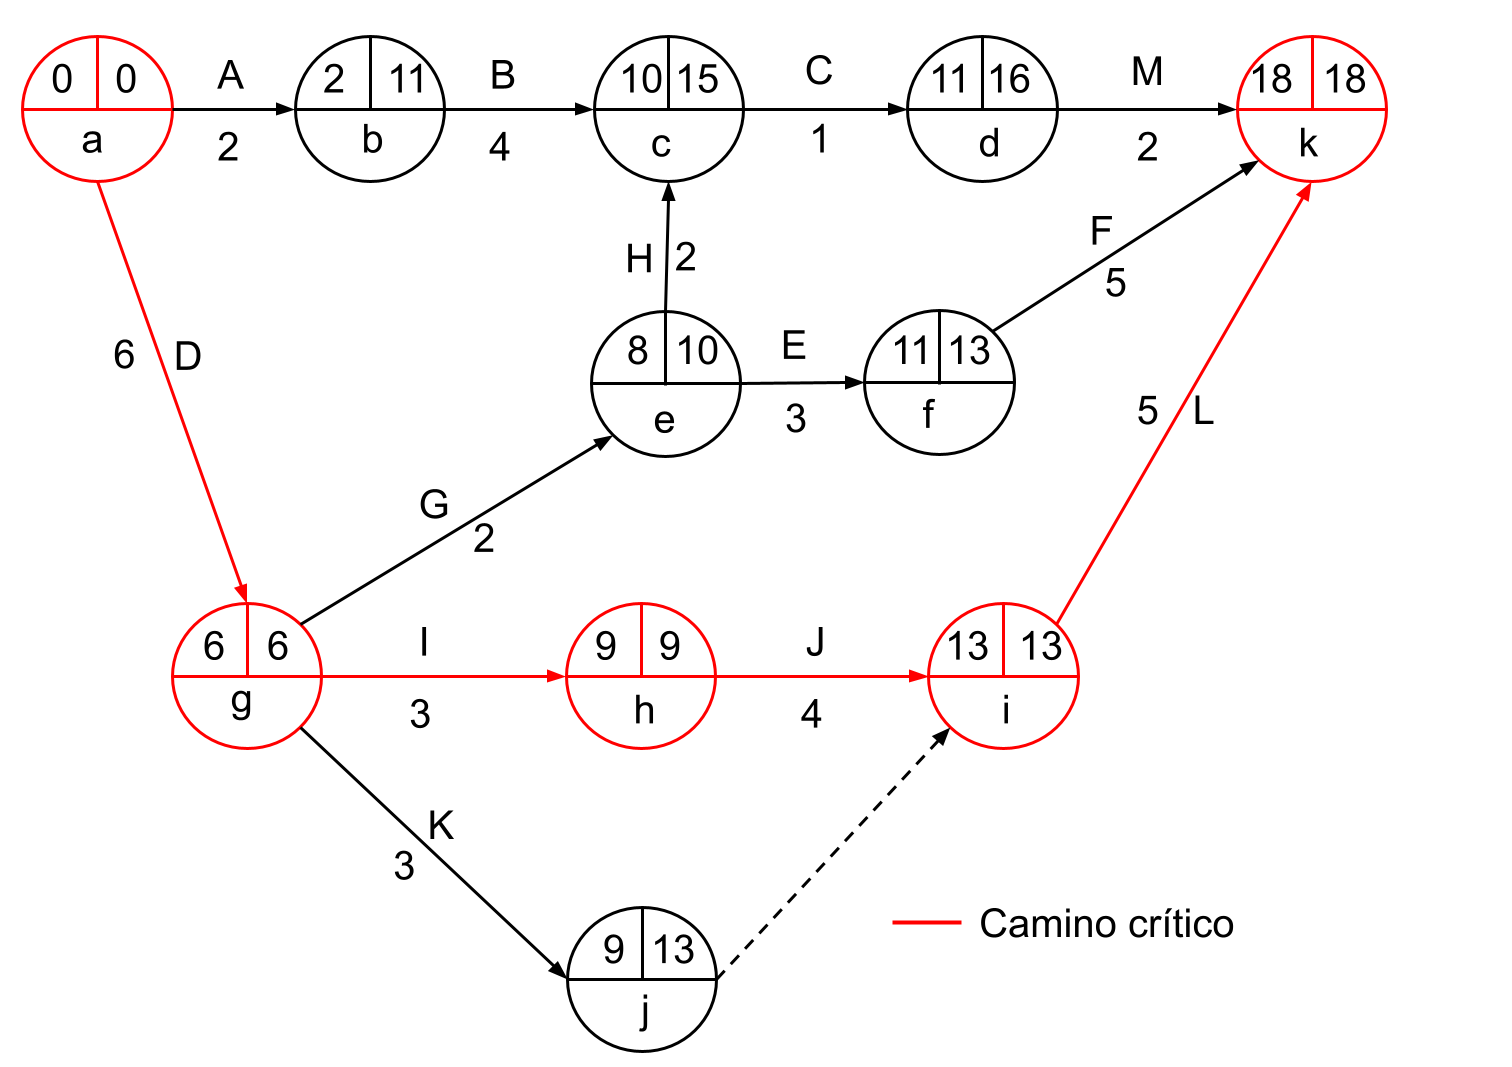
\includegraphics[scale=0.3]{../figures/pert_01.png}

    \item Matriz asociada al grafo
    
    \begin{center}
    \begin{tabular}{c|cccccccccccccc}
          & A & B & C & D & E & F & G & H & I & J & K & L & M \\
      \hline
        A   & 0 & 0 & 0 & 0 & 0 & 0 & 0 & 0 & 0 & 0 & 0 & 0 & 0 \\
        B   & \textcolor{red}{1} & 0 & 0 & 0 & 0 & 0 & 0 & 0 & 0 & 0 & 0 & 0 & 0 \\
        C   & 0 & \textcolor{red}{1} & 0 & 0 & 0 & 0 & 0 & \textcolor{red}{1}& 0 & 0 & 0 & 0 & 0 \\
        D   & 0 & 0 & 0 & 0& 0& 0& 0& 0& 0& 0& 0& 0& 0 \\
        E   & 0 & 0 & 0 & 0& 0& 0& \textcolor{red}{1}& 0& 0& 0& 0& 0& 0 \\
        F   & 0 & 0 & 0 & 0& \textcolor{red}{1}& 0& 0& 0& 0& 0& 0& 0& 0 \\
        G   & 0 & 0 & 0 & \textcolor{red}{1}& 0& 0& 0& 0& 0& 0& 0& 0& 0 \\
        H   & 0 & 0 & 0 & 0& 0& 0& \textcolor{red}{1}& 0& 0& 0& 0& 0& 0 \\
        I   & 0 & 0 & 0 & \textcolor{red}{1}& 0& 0& 0& 0& 0& 0& 0& 0& 0 \\
        J   & 0 & 0 & 0 & 0& 0& 0& 0& 0& \textcolor{red}{1}& 0& 0& 0& 0 \\
        K   & 0 & 0 & 0 & \textcolor{red}{1}& 0& 0& 0& 0& 0& 0& 0& 0& 0 \\
        L   & 0 & 0 & 0 & 0& 0& 0& 0& 0& 0& \textcolor{red}{1}& \textcolor{red}{1}& 0& 0 \\
        M   & 0 & 0 & \textcolor{red}{1} & 0& 0& 0& 0& 0& 0& 0& 0& \textcolor{red}{1}& 0 \\
    \end{tabular}
  \end{center}

    \item ¿Qué efectos tendrán sobre el proyecto los siguientes eventos:

    - La actividad A se retrasa 9 semanas

No afectaría al proyecto puesto que para terminar la actividad A, tenemos
justamente 9 semanas de holgura.

    - La actividad D se retrasa 3 semanas

Dado que la actividad se encuentra en el camino crítico, retrasaría todo el
proyecto 3 semanas.

    - La actividad L se reduce en 1 semana

Esta actividad también se encuentra en el camino crítico y no tiene holgura, por
lo que su retraso tendría como consecuencia el retraso de todo el proyecto.

\end{itemize}

\section{Ejercicio 2}

La empresa CLARK S.A. de C.V. debe reubicar sus oficinas hacia nuevas
instalaciones en la zona norte con el objetivo de brindar una atención
especializada a sus clientes, el director debe preparar un informe detallado de
las labores y el tiempo de cada uno para el traslado, incluyendo rutas críticas
y estimaciones de tiempos. El director ha desarrollado el proyecto con 11
actividades que se presentan en el siguiente cuadro: \\
\\
\begin{center}
  \begin{tabular}{cp{0.18\linewidth}cp{0.1\linewidth}p{0.12\linewidth}p{0.1\linewidth}}
    Actividad   &    Detalle    &   Precedentes & Est. optimista  & Est.
    más probable    &   Est. pesimista    \\
    \hline
      A  & Seleccionar tipo de oficinas & -      &  1    &  3   &  5  \\
      B  & Crear plan organizacional    & -      &  3    &  4.5 &  9  \\ 
      C  & Determinar personal          & B      &  2    &  3   &  4  \\ 
      D  & Diseñar las instalaciones    & A,C    &  2    &  4   &  6  \\ 
      E  & Contruir los interiores      & D      &  4    &  7   &  16 \\
      F  & Seleccionar personal         & C      &  1    &  1.5 &  5  \\
      G  & Contratar nuevos empleados   & F      &  2.5  &  3.5 &  7.5\\
      H  & Traslado de archivos y material & F      &  1    &  2   &  3  \\
      I  & Hacer arreglos financieros   & B      &  4    &  5   &  6  \\
      J  & Capacita nuevo personal      & H,E,G  &  1.5  &  3   &  4.5
  \end{tabular}
\end{center}

\begin{itemize}
    \item Diseño completo del grafo, incluyendo holguras y camino crítico.

    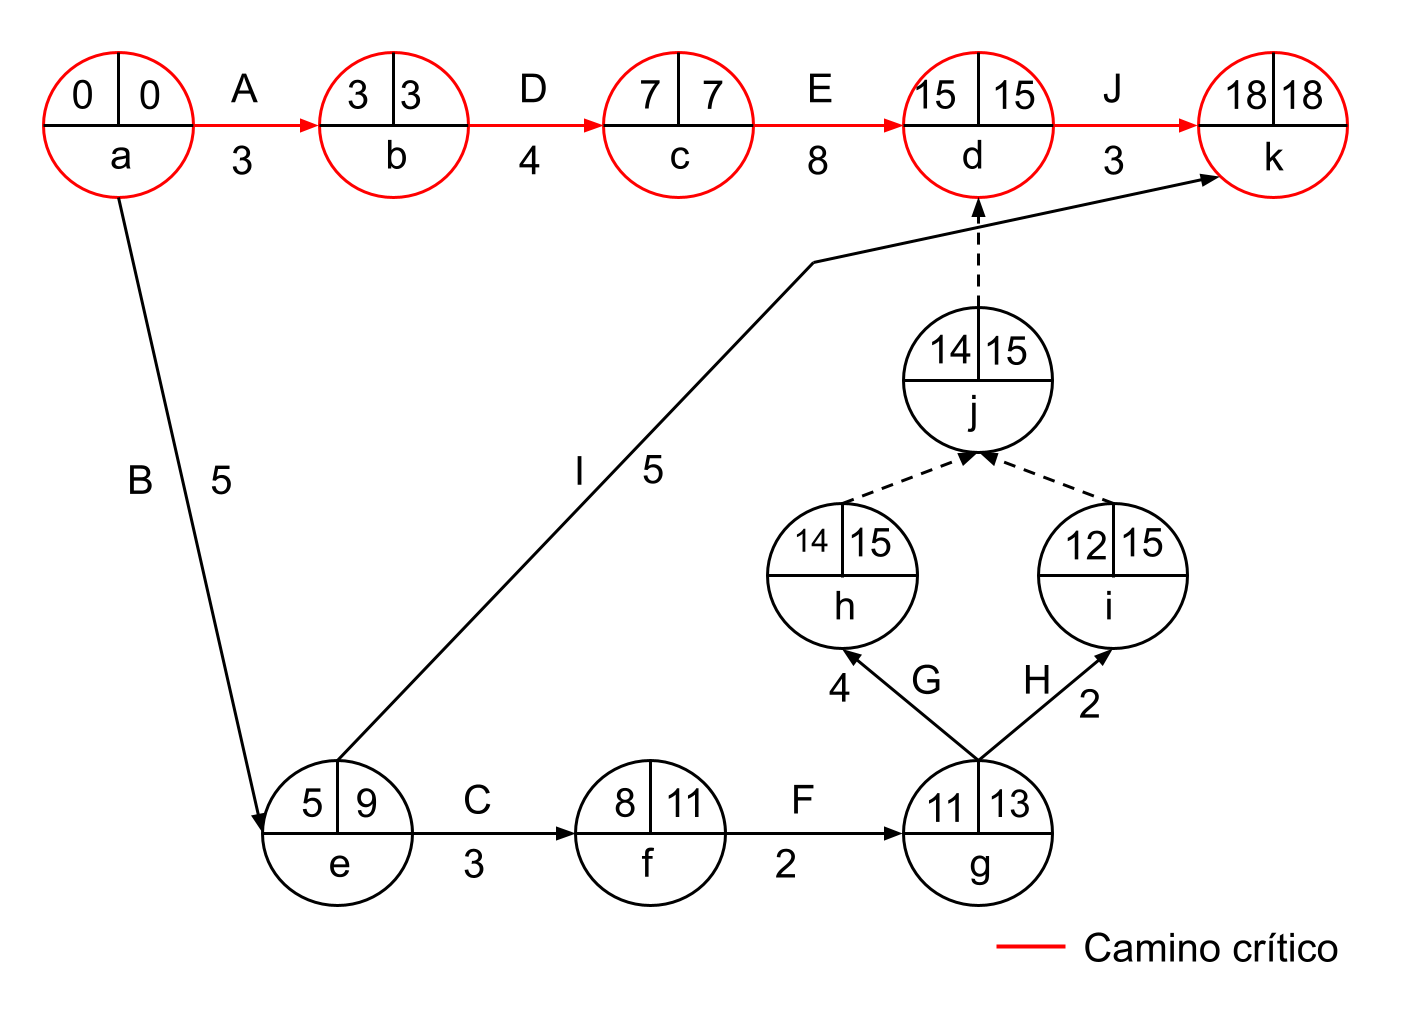
\includegraphics[scale=0.3]{../figures/pert_02.png}

    \item Matriz de encaminamientos asociada al grafo

    \begin{center}
      \begin{tabular}{c|cccccccccc}
             & A & B & C & D & E & F & G & H & I & J \\
        \hline
          A  & 0& 0& 0& 0& 0& 0& 0& 0& 0 & 0 \\
          B  & 0& 0& 0& 0& 0& 0& 0& 0& 0 & 0 \\ 
          C  & 0& \textcolor{red}{1}& 0& 0& 0& 0& 0& 0& 0 & 0 \\ 
          D  & \textcolor{red}{1}& 0& \textcolor{red}{1}& 0& 0& 0& 0& 0& 0 & 0 \\ 
          E  & 0& 0& 0& \textcolor{red}{1}& 0& 0& 0& 0& 0 & 0 \\
          F  & 0& 0& \textcolor{red}{1}& 0& 0& 0& 0& 0& 0 & 0 \\
          G  & 0& 0& 0& 0& 0& \textcolor{red}{1}& 0& 0& 0 & 0 \\
          H  & 0& 0& 0& 0& 0& \textcolor{red}{1}& 0& 0& 0 & 0 \\
          I  & 0& \textcolor{red}{1}& 0& 0& 0& 0& 0& 0& 0 & 0 \\
          J  & 0& 0& 0& 0& \textcolor{red}{1}& 0& \textcolor{red}{1}& \textcolor{red}{1}& 0 & 0 
      \end{tabular}
    \end{center}

    \item Duración estimada del proyecto en días
    \item Responder las siguientes preguntas relacionadas con el proyecto:

    - ¿Cuál será la probabilidad de terminar el proyecto hasta 18 días?

    - ¿Cuál será la probabildad de terminar el proyecto hasta 25 días?

- ¿Cuál será la duración del proyecto para una probabilidad de finalización del
95\%?
    
\end{itemize}

\end{document}
    